 
 \let\negmedspace\undefined
\let\negthickspace\undefined
\documentclass[journal]{IEEEtran}
\usepackage[a5paper, margin=10mm, onecolumn]{geometry}
%\usepackage{lmodern} % Ensure lmodern is loaded for pdflatex
\usepackage{tfrupee} % Include tfrupee package

\setlength{\headheight}{1cm} % Set the height of the header box
\setlength{\headsep}{0mm}     % Set the distance between the header box and the top of the text

\usepackage{gvv-book}
\usepackage{gvv}
\usepackage{cite}
\usepackage{amsmath,amssymb,amsfonts,amsthm}
\usepackage{algorithmic}
\usepackage{graphicx}
\usepackage{textcomp}
\usepackage{xcolor}
\usepackage{txfonts}
\usepackage{listings}
\usepackage{enumitem}
\usepackage{mathtools}
\usepackage{gensymb}
\usepackage{comment}
\usepackage[breaklinks=true]{hyperref}
\usepackage{tkz-euclide} 
\usepackage{listings}
% \usepackage{gvv}                                        
\def\inputGnumericTable{}                                 
\usepackage[latin1]{inputenc}                                
\usepackage{color}                                            
\usepackage{array}                                            
\usepackage{longtable}                                       
\usepackage{calc}                                             
\usepackage{multirow}                                         
\usepackage{hhline}                                           
\usepackage{ifthen}                                           
\usepackage{lscape}
\begin{document}

\bibliographystyle{IEEEtran}
\vspace{3cm}

\title{2.5.28}
\author{EE25BTECH11060 - V.Namaswi}
% \maketitle
% \newpage
% \bigskip
{\let\newpage\relax\maketitle}

\renewcommand{\thefigure}{\theenumi}
\renewcommand{\thetable}{\theenumi}
\setlength{\intextsep}{10pt} % Space between text and floats
\textbf{Question}\\
Find the projection of the vector 
\[
\vec{a} = 2\vec{i} + 3\vec{j} + 2\vec{k}
\]
on the vector 
\[
\vec{b} = 2\vec{i} + 2\vec{j} + \vec{k}.
\]
\textbf{solution}\\
given,
\begin{table}[h!]
\centering
\begin{tabular}{|c|c|c|c|}
\hline
\textbf{Vector} & \textbf{i-component} & \textbf{j-component} & \textbf{k-component} \\
\hline
$\vec{a}$ & 2 & 3 & 2 \\
\hline
$\vec{b}$ & 2 & 2 & 1 \\
\hline
\end{tabular}
\caption{Components of vectors $\vec{a}$ and $\vec{b}$}
\end{table}


Projection of vector $\vec{A}$  on $\vec{B}$ is given by \\
\begin{align}
\frac{\vec{A}^\top\vec{B}}{||\vec{B}^2||}\vec{B}
\end{align}

 \begin{align}
 \implies
\frac{\begin{pmatrix} 2 & 3 & 2 \end{pmatrix}\begin{pmatrix}
    2 \\ 2 \\ 1 \end{pmatrix}}{2^2+2^2+1^2}\vec{B}\\
=\frac{2^2+(3)(2)+(2)(1)}{2^2+2^2+1^2}\begin{pmatrix} 2 \\ 2 \\1 \end{pmatrix}\\
=\frac{12}{9}\begin{pmatrix} 2 \\ 2 \\1 \end{pmatrix}\\ 
=\frac{4}{3}\begin{pmatrix} 2 \\ 2 \\1 \end{pmatrix}\\ 
=\begin{pmatrix}
    \frac{8}{3} \\ \frac{8}{3}  \\    \frac{4}{3}
    \end{pmatrix}
\end{align}

The projection vector is given by $\frac{{8}}{3}\,\mathbf{i} + \frac{8}{3}\,\mathbf{j}+ 
\frac{4}{3}\,\mathbf{k}$


Refer fig
\centering
    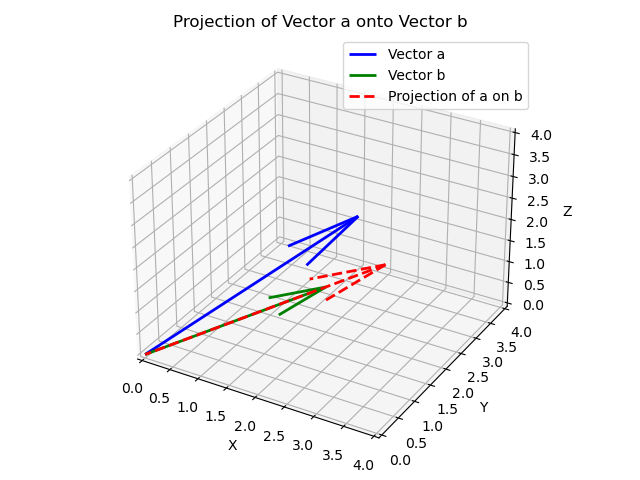
\includegraphics[width=\columnwidth, height=0.8\textheight, keepaspectratio]{figs/Figure_3.png}     

\end{document}